\section{Introduction}

%% 
%% Leave first page empty
\thispagestyle{empty}

The need of a new way to communicate between two points of the planet has been arising as a problem to be solved by our new media distributors. Old systems such as Skype or traditional video calls are not able to cope the needs of the new generations of developers and users that everyday require a more integrated way of communication. 

Besides this, the amount of data being transferred during the last years and the prevision for the future allocates a new scenario where non-centralized systems such as P2P are required as data bandwidth grows and systems need to become more scalable. Nowadays networks are still manly content-centric, meaning that data is provided from a source to a client in a triangle scheme, clients upload data to central servers and this data is transferred to the endpoint. This architecture has been provided since long time as reliable and scalable, but with the appearance of powerful applications and media transfer it has been proven to become a real problem.

Those circumstances lead to a whole new world of real-time browser based applications which require also a totally new framework to be developed into. Starting from the online videoconferencing to real-time data applications, for this purpose few attempts where made in the past being highly reliable on specific hardware and custom-built no-compatible system. Taking these decisions made those proposals not be accessible by the massive amount of normal users that could not afford to adapt the requirements. 

All the previous concepts are now possible thanks to the increase of performance related to the hardware components available in every 
average computer nowadays, this increase has helped to build more complex browsers that are able to perform many tasks not just related 
to web browsing. Having a browser handling OpenGL style of applications is now possible thank to the increase of performance. Besides this multimedia abilities have also been able to reproduce on those browsers and handling webcam media as html is now a reality. Even dough there are still some issues to be considered before being able to freely communicate between two browsers: there is no common standardized protocol that allows developers to do this. WebRTC goal is to approach this problem to build a simple and standard solution for peer-to-peer browser communication \cite{alvestrandOverview2012}.

Internet bandwidth has helped to take the decision to start integrating peer-to-peer solutions in browsed based applications, this is due the year-by-year increase of user bandwidth connectivity during the last 10 years. As before the latency was too high being unable to maintain real-time applications working resiliently. But recently the amount of users being able to transfer at high speed has been rapidly increasing as you can see in Figure ~\ref{fig:bwWorldAvg}, about 39\% of users are now able to download at speeds greater than 4Mbps being this a very good average speed for media content \cite{akamaiq2}.

\begin{figure}[h]
  \centering
    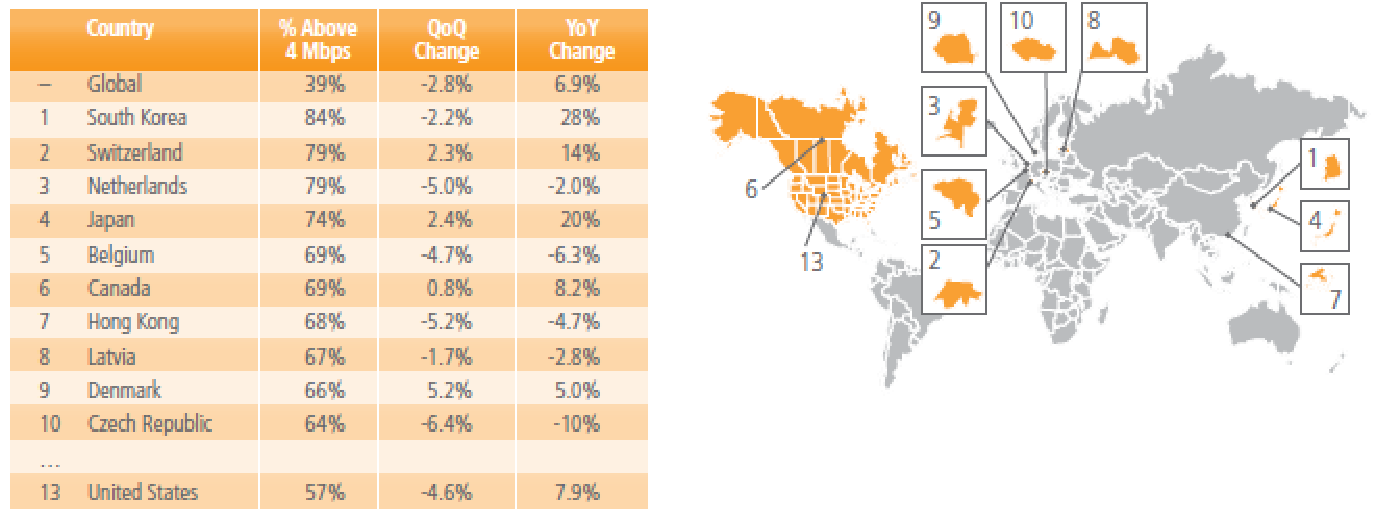
\includegraphics[width=1\textwidth]{./figures/internetstats.pdf}
      \caption[Broadband over 4Mbps connectivity statistics]{Broadband connectivity statistics about the speeds over 4Mbps around the globe.}
	\label{fig:bwWorldAvg}
\end{figure}

Regarding the specs on the client side, recent surveys and statistics taken by the game manufacturer Steam  \cite{steamStats} has proven that nowadays more than  61\% of machines are carrying 1 to 4 gigabytes of RAM and nearly 90\% of computers are handling 2 to 4 core CPU with a 64 bit OS, being this environment optimistic for media enhanced applications which require high performance for video encoding and similar. Due to the layering needed to standardize a system like WebRTC running in top of an underlying application such as the browser that handles many processes is very important to rely on a powerful machine. Usually this was not able to be done in the past and one of the challenges has always been performance. They key to success is always to optimize the performance of a process so it does not affect the user experience, one of the challenges of WebRTC.

Traditionally, this concept of performance was approached by the usage of plug-ins or other separate software components which made the system run smoother by avoiding one layer of processing (browser) but being non-standard and not cross-compatible, one of the most import ant concepts when designing applications nowadays. Now the traditional approach has become outdated with the arrival of the new HTML5 where WebRTC is integrated as one of the new APIs available alongside other many different interesting approaches.

\subsection{History}

Web Real-Time Communication is an API definition with the aim to start an interoperability standard that will help to build P2P applications in the developer layer. The first announcement concept went public in a working group of the World Wide Web Consortium (W3C) in May 2011 \cite{webrtcW3cgroup} and starting the mailing list in April 2011 \cite{welcomeW3C}. During the first stage of the working group the main goal was to define a public draft for the API implementation and a route timeline with the goal to standardize the protocol by ends of 2012. The first public draft of the W3C came public the 27th of October 2011 written by Adam Bergkvist (Ericsson), Daniel C. Burnett (Voxeo), Cullen Jennings (Cisco) and Anant Narayanan (Mozilla) \cite{originalW3Cdraft}. During this first W3C draft only media (audio and video) where considered as candidates to be sent over the network to other peers, manly focusing in the way browsers will be able to access the media devices without using any plugin or external software.

Parallely to the W3C working group the WebRTC concept also joined the IETF with a working group in May 2011 \cite{webrtcIETFgroup} with the first public announcement charter done the 3th of May 2011 by Magnus Westerlund (Ericsson), Cullen Jennings (Cisco) and Ted Hardie (Ericsson). The milestones of the working group charter initially marked December of 2011 to provide the information and elements required to the W3C for the API design input. On the other side, the main goals of the working group covered the definition of the communication model, session management, security, NAT traversal solution, media formats, codec agreement and transport of the data \cite{webrtcIETFcharter}. Those goals have been evolving during the standardzation process and the work done along with the W3C working group.

An important point during the process of standardization came the 1st of June 2011 when Google publicly released the source code of their API implementation \cite{haraldpublicWebRTC}. 

During all this period both working groups have been working alongside to provide a reliable solution to enable applications to perform media and data transfer in a plugin-free environment.

\subsection{Support}

The following companies have publicly supported and are actively working in the development of WebRTC standards in the W3C: Google, Mozilla and Opera \cite{googleAnnouncement}. Other companies such as Microsoft have been publicly supporting a browser-to-browser solution but have provided their own proposal which differs with the one published in the WebRTC group \cite{curtcweb}.

\subsection{Milestones}